
\section{Framework}
\subsection{Basics}
\begin{frame}{\large Markov Random Field}
  \framesubtitle{Markov Random Field (MRF) and Fundamental Inference Problems}
  % \onslide<1->{
    
  % }
  \onslide<1->{
    Let us walk through via MRF
    \begin{itemize}[label={$\bullet$}]
    \item An MRF can be represented by a graph $\Gg(\Vv, \Ee)$ with each node $i\in \Vv$ is associated with a random variable $X_i$
    \item The probability distribution (Gibbs distribution) is
      \begin{equation*}\label{eq:joint-px}
        p(\bm{x}; \bm{\theta}) = \frac{1}{Z(\bm{\theta})} \prod_{a} \psi_a(\bm{x}_a; \bm{\theta}_a),
      \end{equation*}
      where $\bm{x}=\left\{ x_1, x_2, \cdots, x_N \right\}$, $a$ indexes potential functions $\Ii=\{\psi_A, \psi_B, \cdots, \psi_M\}$ and $\bm{\theta}$ is set of potential function parameters. $Z(\bm{\theta}) = \sum_{\bm{x}}\prod_{a} \psi_a(\bm{x}_a;\bm{\theta}_a)$.
    \end{itemize}
  }
  
\end{frame}

\subsection{Usage Abstraction}

{ \setbeamercolor{background canvas}{bg=hl_bg}
  \setbeamercolor{normal text}{fg=hl_fg}
  \setbeamercolor{frametitle}{fg=hl_fg}
  \begin{frame}
    \usebeamercolor[fg]{normal text}
    \begin{center}
      {\large What do we do with graphical models?}
    \end{center}
    
  \end{frame}
}

\begin{frame}{Usage of Graphical Models}
  In general:
  \begin{itemize}[label={$\bullet$}]
    \onslide<1->{
    \item Representation\\
      \begin{itemize}[label={$\bullet$}]
      \item In place of real systems 
      \item Abstraction of complex problems or systems (with subjective bias)
      \end{itemize}
    \item Answer queries\\ Evidence (observation) $\rightarrow$ ?? $\rightarrow$ Answers}
    
  \end{itemize}
  \onslide<2->{
    Two components interacting with each other:
    \begin{figure}[!t]
      \centering
      \begin{tikzpicture}
        \tikzstyle{cnode} = [thick, draw=black, ellipse, inner sep = 2pt,  align=center]
        \tikzstyle{fnode} = [thick, draw=black, ellipse, inner sep = 10pt,  align=center]
        
        \node[cnode] (infn) at (0,0) {Inference};
        \node[cnode] (lern) at (3,0) {Learning};
        
        \node[fnode, fit=(infn)(lern)] (box) {};
        \node[] at (1.4, -0.6) {\textbf{Probabilistic} Graphical Model};
        \draw[->,line width=0.2mm] (infn) to[out=15, in=165] (lern);
        \draw[->,line width=0.2mm] (lern) to[out=195, in=-15] (infn);
      \end{tikzpicture}
      
      \label{fig:intro-pgm}
    \end{figure}
  }
  
\end{frame}

\begin{frame}{Usage of Graphical Models}
  Why impact in two direction?


  \begin{itemize}[label=$\bullet$]
    \onslide<1>{
    \item Learning to Inference:\\
      \begin{figure}[!t]
        \centering
        \begin{tikzpicture}
          \tikzstyle{cnode} = [thick, draw=black, ellipse, inner sep = 2pt,  align=center]
          \tikzstyle{fnode} = [thick, draw=black, ellipse, inner sep = 10pt,  align=center]
          
          \node[cnode] (infn) at (0,0) {Inference};
          \node[cnode] (lern) at (3,0) {Learning};
          
          % \node[fnode, fit=(infn)(lern)] (box) {};
          % \node[] at (1.4, -0.6) {Probabilistic Graphical Model};
          \draw[->,line width=0.2mm] (infn) to[out=15, in=165] (lern);
          \draw[green, ->,line width=0.2mm] (lern) to[out=195, in=-15] (infn);
        \end{tikzpicture}
      \end{figure}
      A graphical model
      \begin{itemize}[label=$\bullet$]
      \item built by expert knowledge, or
      \item built by extracting information from evidence (empirical data).
      \end{itemize}
      }
    \onslide<2->{
    \item Inference to Learning:\\
      \begin{figure}[!t]
        \centering
        \begin{tikzpicture}
          \tikzstyle{cnode} = [thick, draw=black, ellipse, inner sep = 2pt,  align=center]
          \tikzstyle{fnode} = [thick, draw=black, ellipse, inner sep = 10pt,  align=center]
          
          \node[cnode] (infn) at (0,0) {Inference};
          \node[cnode] (lern) at (3,0) {Learning};
          
          % \node[fnode, fit=(infn)(lern)] (box) {};
          % \node[] at (1.4, -0.6) {Probabilistic Graphical Model};
          \draw[green, ->,line width=0.2mm] (infn) to[out=15, in=165] (lern);
          \draw[->,line width=0.2mm] (lern) to[out=195, in=-15] (infn);
        \end{tikzpicture}
      \end{figure}
      Model learning: an error trial process that compares inferred 'fact' and actual fact (evidence).\\
      Model learning usually needs inference as a subroutine, which sometimes are replaced by sampling in particle based methods.
    }
  \end{itemize}
  
  
\end{frame}


\begin{frame}{\large Common Inference Problems}
  The common inference problems in a MRF $\Gg(\Vv, \Ee)$:
  \begin{itemize}[label={$\bullet$}]
  \item Computing the likelihood of observed data.
  \item Computing the marginals distribution $p(\bm{x}_A)$ over particular subset $A \subset \Vv$ of nodes
  \item Computing the conditional distribution $p(\bm{x}_A | \bm{x}_{B})$, 
  \item Computing the most likely configuration $\argmax_{\bm{x}} p(\bm{x})$
  \end{itemize}
  \onslide<2>{
  \begin{tikzpicture}[scale=0.9]
    \tikzstyle{nnode} = [rectangle, rounded corners=2pt, inner sep = 2pt,  align=center]
    \tikzstyle{rnode} = [draw=black, rectangle, rounded corners=2pt, inner sep = 2pt,  align=center]

    \node[rnode, opacity=1] (inf) at (0,0) {Inference};
    
    \node[rnode] (apx) at (2,-1) {Approximate/Variational Inference};

    \node[nnode] (e1) at (-3,-2) {Variable Elimination};
    \node[nnode] (e2) at (-3,-3) {BP in Trees};
    \node[nnode] (e3) at (-3,-4) {Junction Tree};
    \node[nnode] (e4) at (-3,-6) {AND/OR search\\ ...};

    \node[rnode, fit=(e1)(e2)(e3)(e4), label=above:{Exact Inference}] (exact) {};
    
    
    
    
    \node[nnode] (sto) at (1,-4) {
      Importance sampling\\
      Rejection sampling (RS) \\
      Adaptive RS \\
      Markov Chain Monte Carlo\\
      Gibbs sampling\\
      ...
    };
    \node[rnode, fit=(sto), label=above:{Stochastic}] {};

    \node[nnode] (d1) at (5.5,-6) {
      Mean field\\
      Loopy belief propagation (BP)  \\
      Tree-reweighted BP\\
      Generalized BP\\
      ...
    };
    \node[nnode] (d2) at (5.5,-4) {
      Assumed density filter \\
      Expectation propagation (EP)  \\
      Tree-structure EP\\
      Stochastic EP\\
      ...
    };

    \node[rnode, fit=(d1)(d2), label=above:{Deterministic}] (det) {};

    \draw[->] (inf) -- (exact);
    \draw[->] (inf) -- (apx);
    \draw[->] (apx) -- (sto);
    \draw[->] (apx) -- (det);

  \end{tikzpicture}
  }
  
  
\end{frame}

\begin{frame}{\large Inference Routine in Learning}
  \onslide<1->{
    What is $\bm{\theta}$ in $p(\bm{x}; \bm{\theta}) = \frac{1}{Z(\bm{\theta})} \prod_{a} \psi_a(\bm{x}_a; \bm{\theta}_a)$? \\
    A direct view:
    \begin{align*}
      \max_{\bm{\theta}} \log{p(\bm{x}; \bm{\theta})} =  \max_{\bm{\theta}}\sum_{a}\log{ \psi_a(\bm{x}_a; \bm{\theta}_a) } \underbrace{- \log{Z(\bm{\theta})}}_{Helmholtz~free~energy},
    \end{align*}
  }
  \onslide<2->{
    An alternative view:
    \begin{align*}
      \pd{\log{p}(\bm{x};\bm{\theta})}{\bm{\theta}_a} = \pd{\log{{\phi_a}(\bm{x}_a; \bm{\theta}_a)}}{\bm{\theta}_a} - \EE_{p(\bm{x}_a; \bm{\theta})}\left[ \pd{\log{{\phi_a}(\bm{x}_a; \bm{\theta}_a)}}{\bm{\theta}_a} \right].
    \end{align*}

    Remark:
    \begin{itemize}[label={$\bullet$}]
    \item This essentially requires estimation of Helmholtz free energy or marginal probabilities.
    \item Stationary points translate into moment matching.
    \end{itemize}
  }
\end{frame}


% \begin{frame}
%   \frametitle{A biased incomplete branching to methods}
%   \begin{tikzpicture}
%     \tikzstyle{nnode} = [rectangle, rounded corners=2pt, inner sep = 2pt,  align=center]
%     \tikzstyle{rnode} = [draw=black, rectangle, rounded corners=2pt, inner sep = 2pt,  align=center]

%     \node[rnode, opacity=1] (inf) at (0,0) {Inference};
    
%     \node[rnode] (apx) at (2,-1) {Approximate/Variational Inference};

%     \node[nnode] (e1) at (-3,-2) {Variable Elimination};
%     \node[nnode] (e2) at (-3,-3) {BP in Trees};
%     \node[nnode] (e3) at (-3,-4) {Junction Tree};
%     \node[nnode] (e4) at (-3,-6) {AND/OR search\\ ...};

%     \node[rnode, fit=(e1)(e2)(e3)(e4), label=above:{Exact Inference}] (exact) {};
    
    
    
    
%     \node[nnode] (sto) at (1,-4) {
%       Importance sampling\\
%       Rejection sampling (RS) \\
%       Adaptive RS \\
%       Markov Chain Monte Carlo\\
%       Gibbs sampling\\
%       ...
%     };
%     \node[rnode, fit=(sto), label=above:{Stochastic}] {};

%     \node[nnode] (d1) at (5,-6) {
%       Mean field\\
%       Loopy belief propagation (BP)  \\
%       Tree-reweighted BP\\
%       Generalized BP\\
%       ...
%     };
%     \node[nnode] (d2) at (5,-4) {
%       Assumed density filter \\
%       Expectation propagation (EP)  \\
%       Tree-structure EP\\
%       Stochastic EP\\
%       ...
%     };

%     \node[rnode, fit=(d1)(d2), label=above:{Deterministic}] (det) {};

%     \draw[->] (inf) -- (exact);
%     \draw[->] (inf) -- (apx);
%     \draw[->] (apx) -- (sto);
%     \draw[->] (apx) -- (det);

%   \end{tikzpicture}
  
% \end{frame}


%%%%%%%%%%%%%%%%%%%%%%%%%%%%%%%%%%%%%%%%%%%%%%%%%%%%%% 
% ------------------------------------------------
%%%%%%%%%%%%%%%%%%%%%%%%%%%%%%%%%%%%%%%%%%%%%%%%%%%%%% 
\section{Inference}
\subsection{Collection of Inference Methods}
{ \setbeamercolor{background canvas}{bg=hl_bg}
  \setbeamercolor{normal text}{fg=hl_fg}
  \setbeamercolor{frametitle}{fg=hl_fg}
  \begin{frame}
    \usebeamercolor[fg]{normal text}
    \begin{center}
      {\large
        Play with
        \textbf{Gibbs (variational) free energy}
        \begin{equation*}
          F_V(b) = \mathrm{KL}(b( \bm{x}) || p(\bm{x}; \bm{\theta})) - \log{Z(\bm{\theta})}
        \end{equation*}
        with trial $b(\bm{x})$.
      }
    \end{center}
    
  \end{frame}
}


\subsection{Intuition of Message Passing}
\begin{frame}{What is the state of $x$?}
  \framesubtitle{A toy example}
  Assume that we are interested into the state of node $i$ in an MRF, it can be answered by
  \begin{itemize}[label={$\bullet$}]
  \item the probability $p(x_i)$, or
  \item an empirical version, a collection of samples $\left\{ x_i^n \right\}_{n=1}^{N}$
  \end{itemize}
  It is similar for the case when $\bm{x}$ is of interests, instead of $x_i$.
  \begin{figure}
    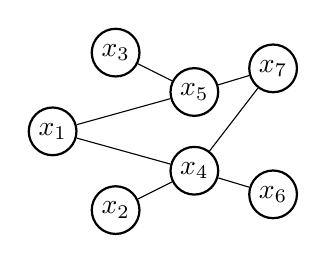
\begin{tikzpicture}
      % \tikzstyle{enode} = [thick, draw=blue, circle, inner sep = 3pt,
      % align=center]
      \tikzstyle{enode} = [thick, draw=black, circle, inner sep = 2pt,  align=center]
      \node[enode] (x1) at (-0.8,0) {$x_1$};
      \node[enode] (x2) at (0,-1) {$x_2$};
      \node[enode] (x3) at (0,1) {$x_3$};
      \node[enode] (x4) at (1,-0.5) {$x_4$};
      \node[enode] (x5) at (1,0.5) {$x_5$};
      \node[enode] (x6) at (2,-0.8) {$x_6$};
      \node[enode] (x7) at (2,+0.8) {$x_7$};

      \draw[-] (x1) to (x4);
      \draw[-] (x1) to (x5);
      \draw[-] (x2) to (x4);
      
      \draw[-] (x3) to (x5);
      \draw[-] (x4) to (x6);
      \draw[-] (x4) to (x7);
      \draw[-] (x5) to (x7);
    \end{tikzpicture}
    \captionsetup{labelformat=empty,justification=centering}
    \caption{what is the state of $x_4$}
    
  \end{figure}
  
\end{frame}

\begin{frame}{What is the state of $x$?}
  \framesubtitle{Gibbs sampling: let us guess by sampling}
  We can approximately sample iteratively: $  x_i \sim p(x_i|\bm{x}_{-i}) \sim p(x_i,\bm{x}_{-i})$
  \begin{figure}
    \begin{subfigure}{0.3\textwidth}
      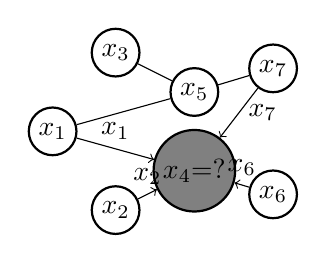
\begin{tikzpicture}
        % \tikzstyle{enode} = [thick, draw=blue, circle, inner sep = 3pt,
        % align=center]
        \tikzstyle{enode} = [thick, draw=black, circle, inner sep = 2pt,  align=center]
        \node[enode] (x1) at (-0.8,0) {$x_1$};
        \node[enode] (x2) at (0,-1) {$x_2$};
        \node[enode] (x3) at (0,1) {$x_3$};
        \node[enode, fill=gray] (x4) at (1,-0.5) {$x_4$=?};
        \node[enode] (x5) at (1,0.5) {$x_5$};
        \node[enode] (x6) at (2,-0.8) {$x_6$};
        \node[enode] (x7) at (2,+0.8) {$x_7$};

        \draw[->] (x1) to node[above] {$x_1$} (x4);
        \draw[-] (x1) to (x5);
        \draw[->] (x2) to node[above] {$x_2$} (x4);
        
        \draw[-] (x3) to (x5);
        \draw[->] (x6) to node[above] {$x_6$} (x4);
        \draw[->] (x7) to node[right] {$x_7$} (x4);
        \draw[-] (x5) to (x7);
      \end{tikzpicture}
      \captionsetup{labelformat=empty,justification=centering}
    \end{subfigure}
    \hskip 0.3in
    \begin{subfigure}{0.3\textwidth}
      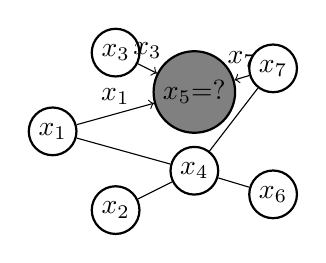
\begin{tikzpicture}
        \tikzstyle{enode} = [thick, draw=black, circle, inner sep = 2pt,  align=center]
        \node[enode] (x1) at (-0.8,0) {$x_1$};
        \node[enode] (x2) at (0,-1) {$x_2$};
        \node[enode] (x3) at (0,1) {$x_3$};
        \node[enode] (x4) at (1,-0.5) {$x_4$};
        \node[enode, fill=gray] (x5) at (1,0.5) {$x_5$=?};
        \node[enode] (x6) at (2,-0.8) {$x_6$};
        \node[enode] (x7) at (2,+0.8) {$x_7$};

        \draw[-] (x1) to (x4);
        \draw[->] (x1) to node[above] {$x_1$} (x5);
        \draw[-] (x2) to (x4);
        
        \draw[->] (x3) to node[above] {$x_3$} (x5);
        \draw[-] (x4) to (x6);
        \draw[-] (x4) to (x7);
        \draw[->] (x7) to node[above] {$x_7$} (x5);
      \end{tikzpicture}
      \captionsetup{labelformat=empty,justification=centering}
    \end{subfigure}
    
  \end{figure}
  This coordinate-wise sampling algorithm is called Gibbs sampling, which answers queries by collected samples $\left\{ \bm{x}^n \right\}_{1}^{N}$.
  \let\thefootnote\relax\footnotetext{\tiny Gibbs sampling is named after the physicist Josiah Willard Gibbs, which was described by brothers Stuart and Donald Geman in 1984, some eight decades after the death of Gibbs.\\
    \begin{equation*}
    x_i \sim \exp\{ \sum_{a \in \mathrm{ne}_i} \log{\phi_{a}}(x_i, \bm{x}_{a-i};\bm{\theta}_{a}) \}
  \end{equation*}
  where $\mathrm{ne}_i$ gives the neighboring potential factors of node $i$.
  }
\end{frame}

\begin{frame}{What is the state of $x$?}
  Naive Mean Field: \textbf{message in form of sample values $\rightarrow$ message in form of belief}
  \begin{figure}
    
    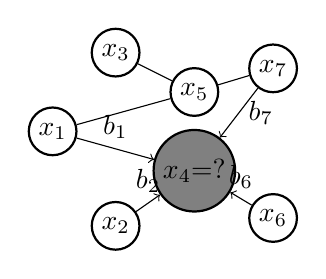
\begin{tikzpicture}
      \tikzstyle{enode} = [thick, draw=black, circle, inner sep = 2pt,  align=center]
      \node[enode] (x1) at (-0.8,0) {$x_1$};
      \node[enode] (x2) at (0,-1.2) {$x_2$};
      \node[enode] (x3) at (0,1) {$x_3$};
      \node[enode, fill=gray] (x4) at (1,-0.5) {$x_4$=?};
      \node[enode] (x5) at (1,0.5) {$x_5$};
      \node[enode] (x6) at (2,-1.1) {$x_6$};
      \node[enode] (x7) at (2,+0.8) {$x_7$};

      \draw[->] (x1) to node[above=0.05mm] {$b_1$} (x4);
      \draw[-] (x1) to (x5);
      \draw[->] (x2) to node[above=0.05mm] {$b_2$}(x4);
      
      \draw[-] (x3) to (x5);
      \draw[->] (x6) to node[above=0.05mm] {$b_6$} (x4);
      \draw[->] (x7) to node[right] {$b_7$} (x4);
      \draw[-] (x5) to (x7);
    \end{tikzpicture}
  \end{figure}
  Corresponding to minimization of \textbf{variational free energy $F_v(b)$  with trial $b$ in fully-factorized form for univariant $\{b_i\}$}.
  \let\thefootnote\relax\footnotetext{\tiny
    Iterative sampling $\rightarrow$ iterative belief update via  
    \begin{equation*}
      \log{b_i(x_i)} \propto \sum_{a \in \mathrm{ne}_i} \sum_{\bm{x}_{a} \backslash x_i} \prod_{j\in {a}\backslash i} b_j(x_j)\log{\phi_{a}}(\bm{x}_{a};\bm{\theta}_{a}).
    \end{equation*}  
  }
\end{frame}

\begin{frame}{What is the state of $x$?}
  \framesubtitle{Belief propagation (BP): let us guess by propagating belief}
  \onslide<1->{

    Proposed by Pearl (1982) for Bayesian networks (tree-structured graphs), which then widely used for general graphs (loopy BP).
    
    {Yedidia, et al, connected the loopy BP with stationary points of \textbf{Bethe free energy}
      \begin{align*}
        F_{Bethe}(b) = \sum_{a\in \Ff} \sum_{\bm{x}_{a}}
        b_{a}(\bm{x}_{a})\log{\frac{b_{a}(\bm{x}_{a})}{\phi_{a}(\bm{x}_{a})}
        } -  \sum_{i=1}^{N} (|\mathrm{ne}_i| - 1) \sum_{x_i} b_i(x_i) \log{b_i(x_i)},
      \end{align*}
    }
    
    Corresponding to minimization of approximated \textbf{variational free energy $F_v(b)$  with trial $b$ includes $\{b_i\}$ and $\{b_a\}$}.

    }
    \let\thefootnote\relax\footnotetext{\tiny
      \vskip -0.8cm
      \begin{align*}
    \mathrm{msg: factor~ to~ variable} ~~ m_{a\rightarrow i}(x_i) & \propto \sum_{\bm{x}_{a} \backslash x_i}
                                \phi_{a}(\bm{x}_{a}) \prod_{j \in a \backslash i} m_{j\rightarrow a}(x_j), \\
    \mathrm{msg: variable~ to~ factor} ~~  m_{j\rightarrow a}(x_j) & \propto  \prod_{a^{\prime} \in \mathrm{ne}_j
                                \backslash a} m_{a^{\prime}\rightarrow j}(x_j)
    \end{align*}
    See, D. Liu, M. T. Vu, Z. Li, and Lars K. Rasmussen. $\alpha$ belief propagation for approximate inference. 2020 \\
    D. Liu, N. N. Moghadam, L. K. Rasmussen, etc. $\alpha$ belief propagation as fully factorized approximation. In
    GlobalSIP, 2019.
    for alternative view to loopy BP.
  }
  
\end{frame}


\begin{frame}{What is the state of $x$?}
  \framesubtitle{Yedidia, Freeman, Weiss: A step to generalization}
  \textbf{Message among variables \& factors $\rightarrow$ message among regions}
  \vskip -0.5cm
  \begin{figure}
    \centering
    \begin{tikzpicture}
      % \tikzstyle{enode} = [thick, draw=blue, circle, inner sep = 3pt,
      % align=center]
      \tikzstyle{enode} = [thick, draw=black, circle, inner sep = 2pt,  align=center]
      \tikzstyle{nnode} = [thick, rectangle, rounded corners = 2pt, minimum size = 0.5cm,draw,inner sep = 2pt]
      \tikzstyle{fnode} = [draw=blue, ellipse, inner sep = 1pt]
      \tikzstyle{fnoder} = [draw=red, ellipse, inner sep = 0.0pt, rotate=-20]


      \node[enode] (x1) at (-1.5, 1) {$x_1$};
      \node[enode] (x2) at (-0.5, 1) {$x_2$};
      \node[enode] (x3) at (0.5, 1) {$x_3$};
      \node[enode] (x4) at (1.5, 1) {$x_4$};

      \node[nnode] (a) at (-2,-1) {A};
      \node[nnode] (b) at (0,-1) {B};
      \node[nnode] (c) at (2,-1) {C};

      \draw[-] (a) to (x1);
      \draw[-] (a) to (x2);
      \draw[-] (b) to (x2);
      \draw[-] (b) to (x3);
      \draw[-] (b) to (x4);
      \draw[-] (c) to (x4);
      
      \node[fnode, fit=(x1)(x2)] (box) {};
      \node[fnoder, fit=(x3)(b)] (box) {};

      \node[fnode, fit=(x2)(x3)(x4)(b)(c)] (box) {};
    \end{tikzpicture}
  \end{figure}
  \vskip -0.5cm
  
  % A region in a region graph acts as a node, and there are directed edges between regions which are defined according to specific rules. Formally, a region graph is defined as follows:

  % A \textit{region graph} is  a directed graph $\Gg_R(\Rr, \Ee)$, where each vertex $R \in \Rr$ is defined as the joint set of variable and factor nodes in this region, i.e., $R = \left\{ i \in V_R, a \in A_R | i \in \Vv, a \in \Ff \right\}$. Each edge $e \in \Ee$ in $\Gg_R$ is directed from $R_p$ to $R_c$ such that $R_c \subset R_p$. 

  Generalized belief propagation (GBP) generalizes loopy BP
  \begin{itemize}[label={$\bullet$}]
  \item usual better approximation than LBP
  \item higher complexity
  \item sensitive to scheduling of region messages
  \end{itemize}
  Corresponding to minimization of approximated \textbf{variational free energy $F_v(b)$  with trial $b$ including $\{b_R\}$}.
  \let\thefootnote\relax\footnotetext{\tiny
    \vskip -0.2cm
    A \textit{region} $R$ is a set $V_R$ of variables nodes and a set $A_R$ of factor nodes, such that if a factor node '$a$' belongs to $A_R$, all the variables nodes neighboring $a$ are in $V_R$.
}
\end{frame}

%%% Local Variables:
%%% mode: latex
%%% TeX-master: "../ppgm_slide"
%%% End:
